
%(BEGIN_QUESTION)
% Copyright 2007, Tony R. Kuphaldt, released under the Creative Commons Attribution License (v 1.0)
% This means you may do almost anything with this work of mine, so long as you give me proper credit

When multiple control valves throttle fluid flow to different points of use from the discharge of a common pump, a control system optimizing pump speed (for minimal energy consumption) needs to incorporate a computational relay, or function block, as shown here:

$$\includegraphics[width=15.5cm]{i01785x01.eps}$$

Explain how this control system works to minimize pumping energy, and what the specific purpose of the relay is.  Also, identify the actions (direct or reverse) of each controller in this system assuming signal-to-open control valves and a signal-to-speed motor drive.

\vskip 20pt \vbox{\hrule \hbox{\strut \vrule{} {\bf Suggestions for Socratic discussion} \vrule} \hrule}

\begin{itemize}
\item{} A useful analytical technique for any complex control system is to annotate the diagram with ``+'' and ``$-$'' symbols at the instrument bubble inputs, designating ``noninverting'' and ``inverting'' characteristics, respectively.  Show how this helps you track of all directions of action, making it easier to figure out how the control system responds to changes.
\item{} Explain what would happen if one of the control valves failed in its wide-open position, despite the efforts of its flow controller to limit flow.
\end{itemize}

\underbar{file i01785}
%(END_QUESTION)





%(BEGIN_ANSWER)

$$\includegraphics[width=15.5cm]{i01785x02.eps}$$

Here, the pump speed is controlled according to the position of the {\it furthest-open} control valve.

%(END_ANSWER)





%(BEGIN_NOTES)

Note: this control strategy derived from diagram on page 127 of Francis G. Shinskey's {\it Energy Conservation Through Control}, copyright 1978.

%INDEX% Control, strategies: valve position optimization
%INDEX% Relay, computational: high select (used in valve position optimization process)

%(END_NOTES)


